\documentclass{beamer}
% \setbeameroption{show notes}
\setbeamerfont{framesubtitle}{size=\normalfont\large}
\setbeamertemplate{footline}[frame number]
\setbeamertemplate{navigation symbols}{}

\usepackage[utf8]{inputenc}
\usepackage[T1]{fontenc}
% \usepackage[ngerman]{babel}

\usepackage{multicol}
\usepackage{prooftree}
\usepackage{bcprules}
\usepackage{scalefnt}
\usepackage{adjustbox}
\usepackage{wasysym}

\usepackage{amssymb}
\usepackage{parskip}
\usepackage{listings}
\usepackage{graphicx}

\usepackage{todonotes}
\let\todox\todo
\renewcommand\todo[1]{\todox[inline]{#1}}

% Turnstile
\newcommand{\ts}{\,\vdash\,}


\title{\\\emph{A Theory of Type Qualifiers}\\ 
\small{}Jeffrey S. Foster, Manuel Fähndrich, Alexander Aiken\\
PLDI 1999}
\author{Paper presentation by\\Georg Schmid and Samuel Grütter}
\date{May 20, 2015}

\begin{document}
\maketitle

\begin{frame}{Overview}
  \begin{itemize}
  \item Many languages support a range of \emph{type qualifiers} -- 
    they enable a simple, yet useful form of subtyping.\\
    \begin{itemize}\item E.g.\ \textsc{const} on references, \textsc{nonzero} on integers.\end{itemize}

  \item Authors present a framework for adding type qualifiers to $\lambda$-calculi.

  \item In particular, they show how to
    \begin{itemize}
    \item extend the typing rules, and
    \item support type inference --
    \item even in the polymorphic case.
    \end{itemize}
  \end{itemize}
\end{frame}


\defverbatim{\lstcduplicateprocs}{%
\begin{lstlisting}[language=C,frame=single,belowskip=- \medskipamount]
int *id1(int *x) { return x; }
const int *id2(const int *x) { return x; }
\end{lstlisting}}

\begin{frame}[fragile]{Motivation}
  \begin{itemize}
  % \item Paper's presentation is closely tied to \textsc{const} qualifier in C
  %   \begin{itemize}\item What are the semantics of \textsc{const} in C?\end{itemize}

  \item<1-> Use-case: Analyze C sources and infer additional \textsc{const} qualifiers

  \item<2->
    This rectifies one particular peculiarity of C's type system:
    % \vspace{1em}
    \lstcduplicateprocs
    $\rightarrow$ Inference of \textsc{const} qualifiers removes need for multiple versions of same procedure
  \end{itemize}
\end{frame}


% \begin{frame}{Preliminaries}{Basic syntax / notation / definitions}
%   \begin{itemize}
%   \item type constructor, $\mathit{Typ}$ (paper\_typ.png), type environment
%   \item framework allows mapping of source lang to lang with qualifiers; paper's source language (paper\_sourcelang)
%   \item qualifiers, pos./neg. (paper\_negposqualifier), negation of a qualifier
%   \item qualifier lattice (paper\_qualifierlattice\_\{def,sample\})
%   \item intuition on qualifier lattice: losing ``information''/capabilites as we move up the lattice
%   \end{itemize}
%   \todo{Split into multiple slides and expand}
% \end{frame}

% \note[itemize]{%
%   \item\emph{Q:} What is a two-point lattice?\\
%   \item\emph{Q:} What is $\bot$ of this lattice? What is $\top$?\\
%   \item\emph{Q:} ``Subset contradiction'' wrt.\ $\tau \subseteq \text{const}\ \tau$ (cf.\ dual notation as negative qualifier ``writable'' / consider \textsc{const} as ``read-only'' / rewrite as ``ConstInt'' $\geq$ ``NormalInt'' class hierarchy)\\
% ``WritableInt'' $\preceq$ ``NormalInt''}

\begin{frame}{Preliminaries}{Qualifiers}
  %
  \begin{center}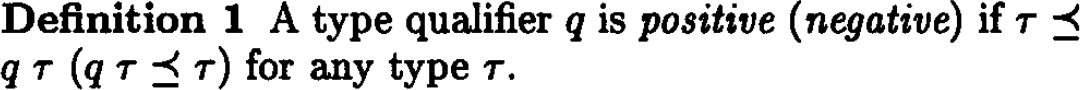
\includegraphics[scale=0.25]{paper_qualifier_def.png}\end{center}
  \begin{itemize}
  \item E.g. \textsc{const} is a positive qualifier, while
    \textsc{nonzero} is negative.
  \end{itemize}

  \bigskip

  \visible<2->{
  \begin{center}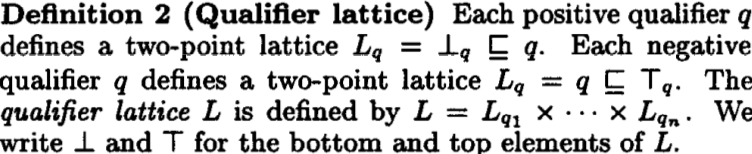
\includegraphics[scale=0.36]{paper_qualifierlattice_def.png}\end{center}
  \begin{itemize}
  \item[$\Rightarrow$] Question: What is a two-point lattice?
  % NOTE: Answered verbally
  \end{itemize}
  }
\end{frame}

\begin{frame}{Preliminaries}{Qualifiers (2)}
  \begin{itemize}
  \item Let's look at the lattice of positive qualifiers \textsc{const}, \textsc{dynamic} and (negative) \textsc{nonzero}: 
    \begin{center}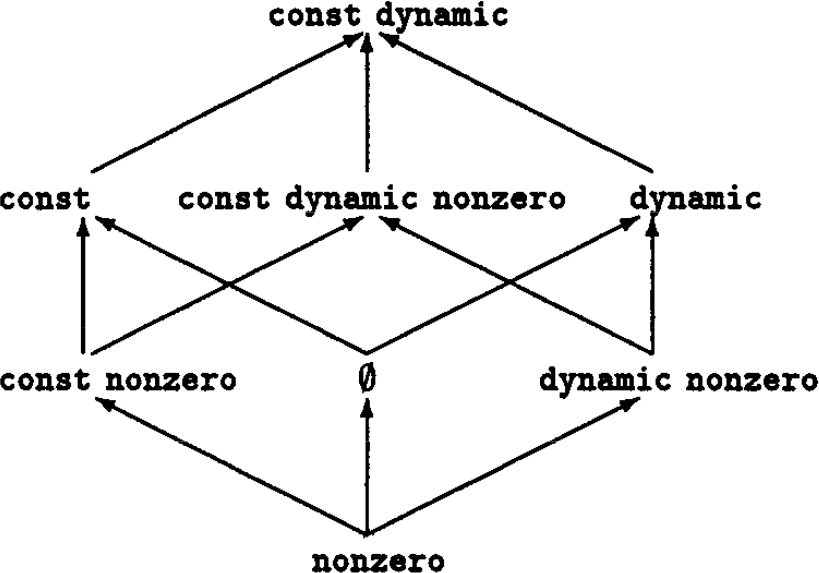
\includegraphics[scale=0.25]{paper_qualifierlattice_sample.png}\end{center}
  \item<2-> Question: What is the $\bot$ of this lattice? What is $\top$?\\
    \visible<3->{Answer: $\bot = \text{``nonzero''}, \top = \text{``const dynamic''}$}
  \end{itemize}
\end{frame}

\begin{frame}{Preliminaries}{Qualifiers (3)}
  \begin{itemize}
  \item How should we interpret $\tau \preceq \text{const}\,\tau$?
    \begin{itemize}
    \item<2-> Assuming $\preceq$ corresponds to $\subseteq$, ``int $\preceq$ const int'' means\\ ``(set of all ints) $\subseteq$ (set of all const ints)''.\\
    So each int is constant, all data immutable!?
    \item<3-> Rather, think of \textsc{const} as \emph{readonly}.\\ Alternatively, consider the qualifier $\text{writable}\ \tau \preceq \tau$ which is dual notation for \textsc{const}.
      % NOTE: Show the interpretation of ReadonlyInt and NormalInt on the board.
    \end{itemize}
  \item<4->[$\Rightarrow$] Intuition: We \emph{lose capabilities} as we move up the lattice.
  \end{itemize}
\end{frame}

\begin{frame}{Preliminaries}{Qualifiers (4)}
  \begin{itemize}
  \item With each qualifier $q_i$ we associate a qualifier lattice element $\neg q_i$, where
    \begin{itemize}
    \item[] $\neg q_i := (\top_1, \dots, \top_{i-1}, \bot_i, \top_{i+1}, \dots, \top_n)$ when $q_i$ is \emph{positive},
    \item[] $\neg q_i := (\bot_1, \dots, \bot_{i-1}, \top_i, \bot_{i+1}, \dots, \bot_n)$ when $q_i$ is \emph{negative}.
    \end{itemize}
  \item<2-> Question: What is $\neg nonzero$?\\
    \visible<3->{Answer: $(\bot_\text{const}, \bot_\text{dynamic}, \top_\text{nonzero}) = \text{\lq\lq}\emptyset\text{''}$}
  \end{itemize}
\end{frame}

% \begin{frame}{Preliminaries}{Qualifiers (2)}
%   \begin{itemize}
%   \item Let's look at the lattice of positive qualifiers \textsc{const}, \textsc{dynamic} and (negative) \textsc{nonzero}:
%   \end{itemize}
%   \begin{columns}[onlytextwidth]
%   \begin{column}{0.5\textwidth}
%     \centering
%     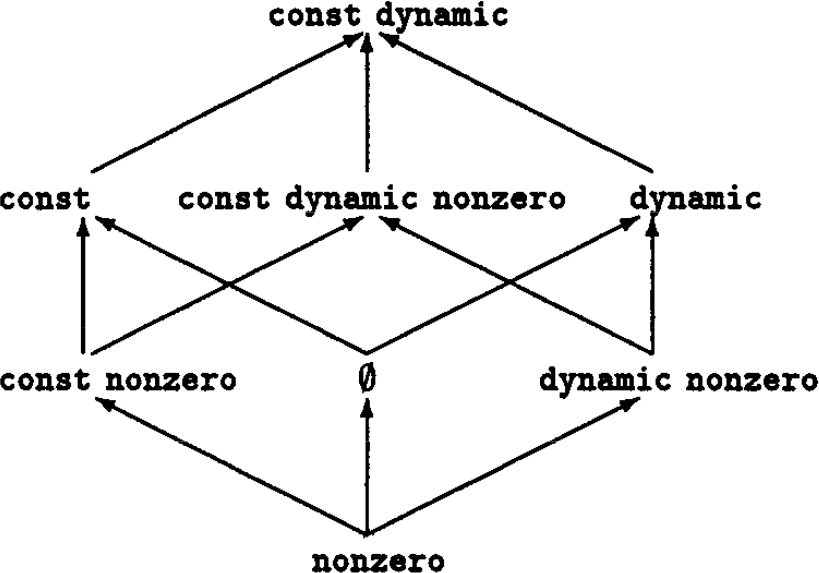
\includegraphics[scale=0.20]{paper_qualifierlattice_sample.png}
%   \end{column}
%   \begin{column}{0.5\textwidth}
%     \begin{itemize}
%     \item<3->[$\Rightarrow$] Q: What is the $\bot$ of this lattice? What is $\top$?
%     \item<4->[$\Rightarrow$] Q: What is $\neg nonzero$?
%       \visible<5-> $(\text{const}, \text{dynamic}, \top_\text{nonzero}) = \text{``const dynamic''}$
%     \end{itemize}
%   \end{column}
%   \end{columns}
%   \begin{itemize}
%   \item<2-> With each qualifier $q_i$ we associate a qualifier lattice element $\neg q_i$, where
%       \begin{itemize}
%       \item[] $\neg q_i := (\top_1, \dots, \bot_i, \dots, \top_n)$ when $q_i$ is \emph{positive}, and
%       \item[] $\neg q_i := (\bot_1, \dots, \top_i, \dots, \bot_n)$ when $q_i$ is \emph{negative}.
%       \end{itemize}
%   \end{itemize}
% \end{frame}

\begin{frame}{Preliminaries}{Source language}
  Framework extends a given source language, e.g.\
  \begin{itemize}
  % \item Types over set of \emph{type constructors} $c \in \Sigma$ and \emph{type variables} $\alpha$:
  %   \begin{center}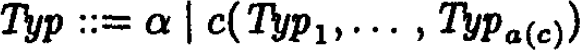
\includegraphics[scale=0.25]{paper_typ.png}\end{center}
  \item Expressions of $\lambda$-calculus with \textsc{if} and \textsc{let}:
    \begin{center}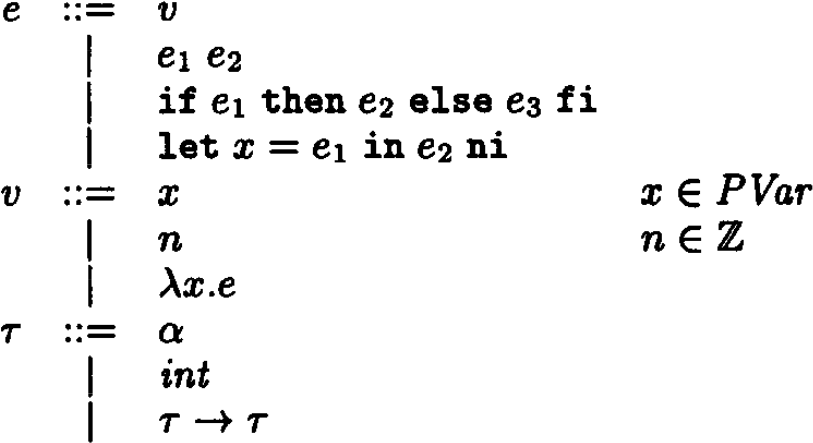
\includegraphics[scale=0.25]{paper_sourcelang.png}\end{center}
  \end{itemize}
\end{frame}

% \begin{frame}{Preliminaries}{Source language}
%   \begin{columns}[onlytextwidth]
%   \begin{column}{0.5\textwidth}
%     \centering
%     %
%   \end{column}
%   \begin{column}{0.5\textwidth}
%     %
%   \end{column}
% ​  \end{columns}
% \end{frame}


\begin{frame}{Qualified types}
  Pairing ordinary types with elements of the qualifier lattice yields \emph{qualified types} for our sample language:
  \begin{center}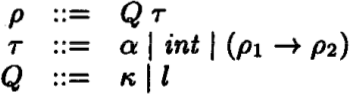
\includegraphics[scale=0.38]{paper_qualifiedtypegrammar.png}\end{center}
  \begin{tabbing}
  \hspace{4em} where \= $\kappa$ is a type qualifier variable and\\
  \> $l$ is an element of qualifier lattice $L$.
  \end{tabbing}

  Along with a pair of subtyping rules that naturally connects the type system to our qualifier lattice:
  \begin{center}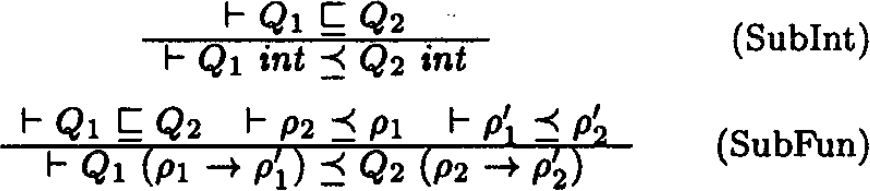
\includegraphics[scale=0.30]{paper_samplelang_subtypingrules.png}\end{center}
\end{frame}


\begin{frame}{Qualifier annotations and assertions}
  \begin{itemize}
  \item When inferring types, we need to decide on a type qualifier for the outermost type constructor.
    \begin{itemize}
    \item \emph{Qualifier annotations} are added as a syntactic helper
      % -- together with the resp.\ typing rule, qualifiers can only increase monotonically (``give up capabilities'')
      % NOTE: Mention this.
    \item Additionally, dual notion of \emph{qualifier assertions}
    \end{itemize}
  \item This requires extensions of both syntax and typing rules:
    \begin{center}
    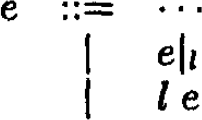
\includegraphics[scale=0.3]{paper_qualifierannass_syntax.png}
    \hspace{1em}\vrule\hspace{1em}
    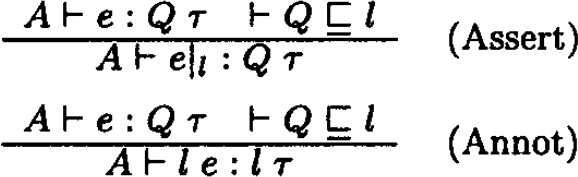
\includegraphics[scale=0.3]{paper_samplelang_annasstyping.png}
    \end{center}
  \item<2-> Both enforce $e$'s top-level qualifier $Q$ to be upper-bounded by $l$, i.e.\ $Q \sqsubseteq l$
    \begin{itemize}
    \item Question: What's the difference between the two?
      % NOTE: Maybe also ask: Which one corresponds to ascription in Scala?
      % NOTE: Follow-up question: What's the difference between Q and l?
    \end{itemize}
  \end{itemize}
\end{frame}

% \note[itemize]{%
%   \item\emph{Q:} What's the difference between assertions and annotations? (Hint: Show typing rules)\\
%   \item\emph{Q/Follow-up:} What's the difference between Q and l?}


\begin{frame}{Qualified type systems}
  \begin{center}\Large
  \begin{tabular}{l c r}
    $A \vdash e : \tau$ & $\Rightarrow$ & $A \vdash e : \rho$
  \end{tabular}
  \end{center}

  \vspace{1em}
  \large
  Extending the source language's type checking system with qualified types leads to a \emph{qualified type system}.
\end{frame}

\begin{frame}{Qualified type systems}{Typing rules of sample language (1)}
  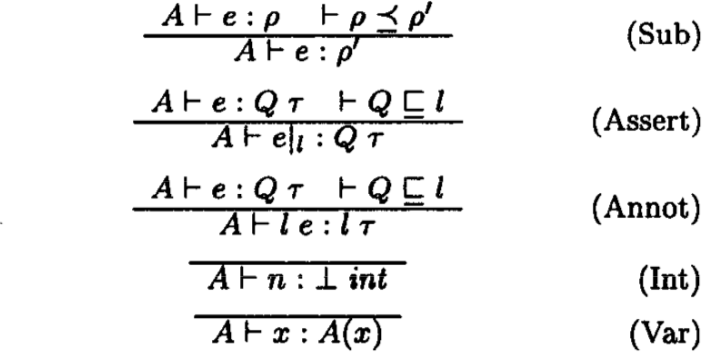
\includegraphics[scale=0.4]{paper_samplelang_typingrules1.png}
\end{frame}

\note[itemize]{%
  \item Discuss how terminal expressions are assigned type qualifier $\bot$.}

\begin{frame}{Qualified type systems}{Typing rules of sample language (2)}
  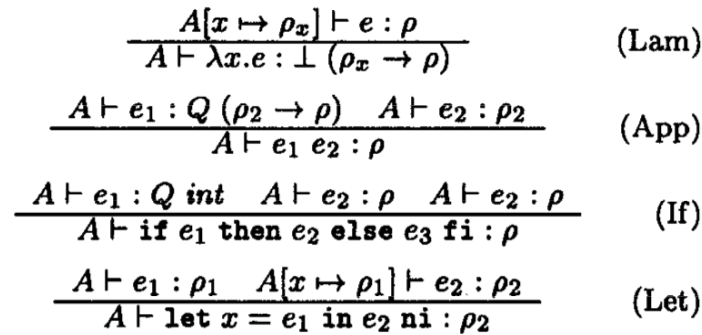
\includegraphics[scale=0.4]{paper_samplelang_typingrules2.png}
\end{frame}

\note[itemize]{\item Discuss unrestricted type qualifier $Q$ in premises.
  \item\emph{Q:} Ad $(\text{App})$. What role do qualifiers on abstractions play in this paper?}


\begin{frame}{Qualified type systems}{Correspondence}
  \begin{itemize}
  \item Type qualifiers should only refine type information,\\ but \emph{not} modify type structure.
  \item[$\Rightarrow$] Correspondence of the original and resp.\ qualified type system
  \item<2-> Helpers:\\
    \begin{itemize}
    \item $\text{strip}(\cdot): \mathit{QTyp} \rightarrow \mathit{Typ}~~$ eliminates qualifiers from types\\
      \visible<3->{\vspace{0.5em}
        Example: $\text{strip}(\,\overline{\bot(\text{const}\ \text{int} \to \text{nonzero}\ \text{int})}\,) =
         \overline{(\text{int} \to \text{int})}$
        }
    \item $\bot(\cdot): \mathit{Typ} \rightarrow \mathit{QTyp}~~$ introduces $\bot$ qualifiers in types\\
      \visible<4->{\vspace{0.5em}
        Example $\bot(\,\overline{(\text{int} \to \text{int})}\,) =
          \overline{\bot(\bot\ \text{int} \to \bot\ \text{int})}$
        }
    \item<5-> $\text{strip}(\cdot): \mathit{Expr} \rightarrow \mathit{Expr}~~$ eliminates annotations \& assertions\\
    \item<5-> $\bot(\cdot): \mathit{Expr} \rightarrow \mathit{Expr}~~$ introduces $\bot$ qualifier annotations everywhere
    \end{itemize}
  % \item[]<2->
  %   \begin{center}
  %   \vspace{1em}
  %   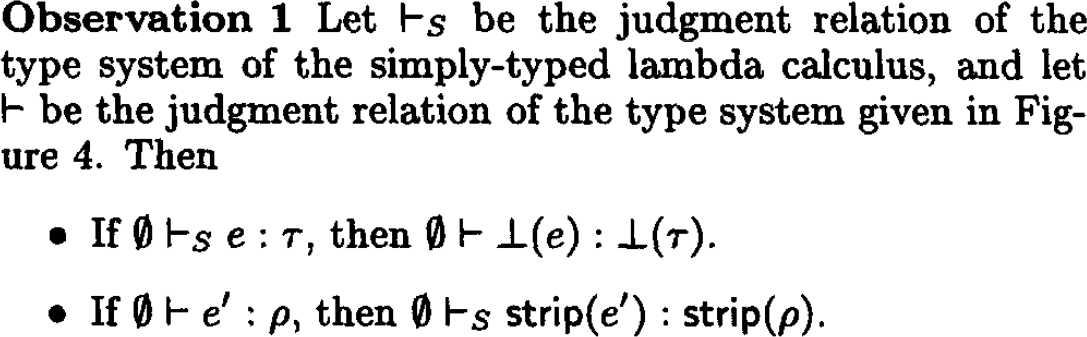
\includegraphics[scale=0.25]{paper_observation1.png}
  %   \end{center}
    %\visible<4->{done{Verify that this is line with the paper's definition of $\bot(\cdot)$.}}
  \end{itemize}
\end{frame}

% \note[itemize]{%
%   \item Discuss definition of $\bot(\cdot)$ and $\text{strip}(\cdot)$.}

\begin{frame}{Qualified type systems}{Correspondence (ctd.)}
  \begin{center}
  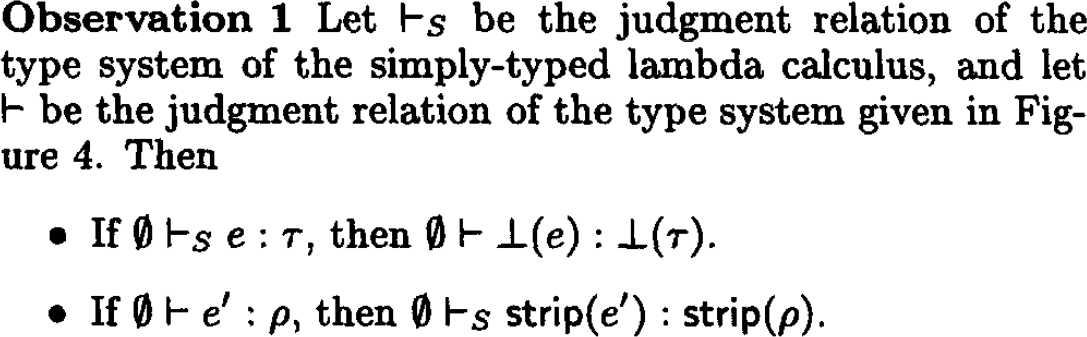
\includegraphics[scale=0.25]{paper_observation1.png}
  \end{center}

  \bigskip
  \begin{itemize}
  \item<2-> Question: Could we use $\top$ instead? Any other qualifier?
  \end{itemize}
\end{frame}

% \note[itemize]{%
%   \item\emph{Q:} Ad $\bot(\cdot)$. Could we use $\top$ instead? Any other qualifier?\\\quad$\rightarrow$ Here, the choice of qualifier is unimportant.}


\begin{frame}{Qualifier semantics}
  \begin{itemize}
  \item Restrictions on usage of qualifiers can be expressed
    \begin{enumerate}[a)]
    % \item using qualifier assertions (injected during a preprocessing step of programs), or
    \item using qualifier assertions ($\rightarrow$ program transformation), or
    \item by modifying typing rules.
    \end{enumerate}
  \item Arbitrary modifications may render the type system unsound!
  \end{itemize}
\end{frame}

\begin{frame}{Qualifier semantics}{\textsc{const} example}
  \begin{itemize}
  \item Let's encode the semantics of a \textsc{const} qualifier!
  \item<2-> Only makes sense in presence of \emph{references}:
    \begin{center}
    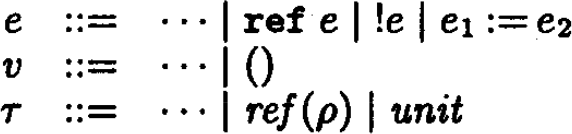
\includegraphics[scale=0.3]{paper_ref_syntax.png}
    \end{center}
  \end{itemize}
\end{frame}

\note{\emph{Q:} Why do they introduce unit / $()$? (Hint: Why only along with references?)}

\begin{frame}{Qualifier semantics}{\textsc{const} example (2)}
  \begin{itemize}
  \item We first introduce a subtyping rule for \textsc{ref}:
    \begin{center}
    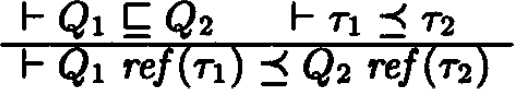
\includegraphics[scale=0.29]{paper_ref_unsound.png}
    \end{center}
  \item<2-> Unsound in the presence of subtyping!
    \begin{center}
    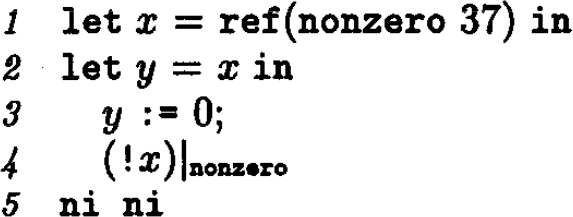
\includegraphics[scale=0.3]{paper_ref_unsoundsample.png}
    \end{center}
  \item<3->[$\Rightarrow$] Note that lines 3 and 4 type check, e.g.\
    \begin{minipage}[t]{0.3\textwidth}
    \begin{tabbing}
    \=\#3: \=$A[x, y \mapsto \bot\,\text{ref nonzero int}]\,\vdash y : \neg\text{nonzero int}$\quad \=\small(by $(\text{Sub})$)\\
    \>\#4: \>$A[x, y \mapsto \bot\,\text{ref nonzero int}]\,\vdash\ !x : \text{nonzero int}$ \>\small(unchanged)
    \end{tabbing}
    \end{minipage}
  \end{itemize}
\end{frame}

\begin{frame}{Qualifier semantics}{\textsc{const} example (3)}
  \begin{itemize}
  \item Requiring refs' argument type to be invariant fixes our problem.
    \begin{center}
    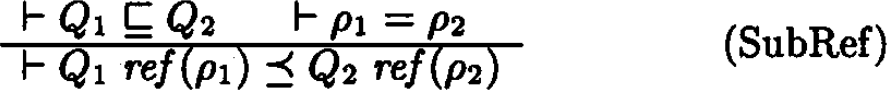
\includegraphics[scale=0.29]{paper_ref_sound.png}
    \end{center}
  % \item<2-> Generally, subtyping rules of the form
  %   \begin{center}
  %   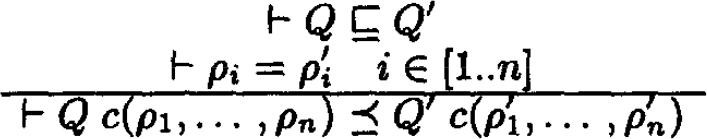
\includegraphics[scale=0.3]{paper_subtypingrule_general.png}
  %   \end{center}
  %   are sound.
  \end{itemize}
\end{frame}

\begin{frame}{Qualifier semantics}{\textsc{const} example (4)}
  \begin{itemize}
  \item How do we enforce the semantics of \textsc{const}?
  \item<2-> As mentioned before, there are two ways to encode such restrictions:
    \begin{enumerate}[a)]
    \item<2-> Program transformation:\\ Replace every assignment $e_1\!:=\!e_2$ by $e_1\!\mid_{\neg\text{const}}\,:=\!e_2$.
    \item<3-> Modify the relevant typing rule(s):\\
      \begin{center}
      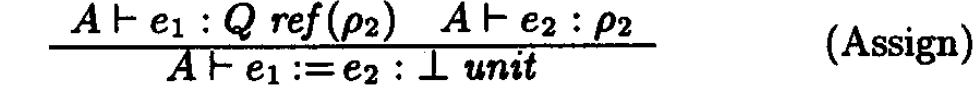
\includegraphics[scale=0.25]{paper_assign_original.png}\\
      \vspace{0.5em}{\Huge $\Downarrow$}\hspace{5.8em}\vspace{0.5em}\\
      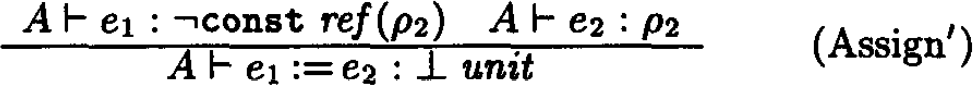
\includegraphics[scale=0.25]{paper_assign_adapted.png}
      \end{center}
    \end{enumerate}
  % \item<2-> Generally, subtyping rules of the form
  %   \begin{center}
  %   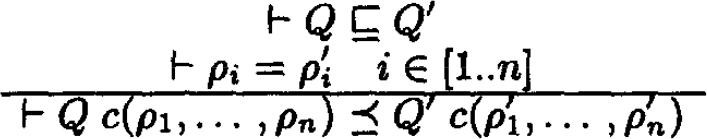
\includegraphics[scale=0.3]{paper_subtypingrule_general.png}
  %   \end{center}
  %   are sound.
  \end{itemize}
\end{frame}

%%%%%%%%%%%%%%%%%%%%%%% SECTION 3 & 4 %%%%%%%%%%%%%%%%%%%%%%%%%%%%%%%%%%%%%%%%%%


\begin{frame}{Type Inference and Qualifier Polymorphism}
Outline
\begin{enumerate}
\item Forget about qualifiers\\
Study type inference on simply typed lambda calculus
%This looks like a mental note to the speaker. -- No it's not ;-)
\item Add qualifiers
\item Add polymorphism
\end{enumerate}
\end{frame}

\begin{frame}{Step 1: Forget about qualifiers}

\infrule[Int]
{}
{A \ts n : int}

\infrule[Var]
{}
{A \ts x : A(x)}

\infrule[Lam]
{A[x \rightarrow \tau_1] \ts e : \tau_2}
{A \ts \lambda x . e : \tau_1 \rightarrow \tau_2}

\infrule[App]
{A \ts e_1 : \tau_2 \rightarrow \tau ~~~~ A \ts e_2 : \tau_2}
{A \ts e_1 e_2 : \tau}

\infrule[If]
{A \ts e_1 : int ~~~~ A \ts e_2 : \tau ~~~ A \ts e_3 : \tau}
{A \ts \text{\textbf{if }} e_1 \text{\textbf{ then }} e_2 \text{\textbf{ else }} e_3 \text{\textbf{ fi}} : \tau}

\infrule[Let]
{A \ts e_1 : \tau_1 ~~~~ A[x \rightarrow \tau_1] \ts e_2 : \tau_2}
{A \ts \text{\textbf{let }} x = e_1 \text{\textbf{ in }} e_2 \text{\textbf{ ni}} : \tau_2}

\end{frame}

\begin{frame}{The problem}

Say we want to typecheck $\lambda x . <\text{some expression}>$.

Use

\infrule[Lam]
{A[x \rightarrow \tau_1] \ts e : \tau_2}
{A \ts \lambda x . e : \tau_1 \rightarrow \tau_2}

but what $\tau_1$ should we put into $A$?

\end{frame}

\begin{frame}{Solutions}

\begin{itemize}
\item Require users to \textbf{explicitly state argument type}\\
      $\lambda (x: \tau_1). e$ instead of $\lambda x . e$
\item \textbf{Local type inference} using \emph{expected types} (e.g. Scala)
      \texttt{List(1, 2, 3).map(x => x+1)}
\item \textbf{Global type inference} (e.g. ML)\\
  \quad\begin{minipage}[t]{0.3\textwidth}
    \textbf{let} $f = \lambda x .\ x + 1$ \textbf{in}\\
    $\dots$\\
    $myList.map(f)$\\
    $\dots$\\
    $otherList.map(f)$
  \end{minipage}
\end{itemize}

\medskip

$\Longrightarrow$ Study \emph{Constraint-Based Typing}

\end{frame}

\begin{frame}{Constraint-Based Typing}

Approach:
\begin{enumerate}
\item Typecheck using the inference rules\\
      Whenever we don't know what type to choose, pick a fresh type variable $\alpha$ and record the constraints it has to satisfy.
\item Unify the constraints
\end{enumerate}

\bigskip

Constraints = set of equality constraints:

\begin{center}
%$C = \{ \tau_1 = \tau_1', ~ \tau_2 = \tau_2',~ \dots \}$

\includegraphics[scale=0.75]{paper_constraint_grammar.png}
\end{center}

\bigskip

New typing judgement:

\begin{center}
%$A \ts e : \tau ; C$

\includegraphics[scale=0.80]{paper_constraint_judgment.png}
\end{center}

``In environment $A$, $e$ has type $\tau$ for all solutions of constraints $C$.''

\end{frame}

\begin{frame}{Constraint-Based Typing Rules}

\infrule[Int]
{}
{A \ts n : int; \emptyset}

\infrule[Var]
{}
{A \ts x : A(x); \emptyset}

\infrule[Lam]
{\alpha \text{ fresh} ~~~~ A[x \rightarrow \alpha] \ts e : \tau_2 ; C}
{A \ts \lambda x . e : \alpha \rightarrow \tau_2 ; C}

\infrule[App]
{\alpha \text{ fresh} ~~~~ A \ts e_1 : \tau_1 ; C_1 ~~~~ A \ts e_2 : \tau_2 ; C_2}
{A \ts e_1 e_2 : \alpha ; C_1 \cup C_2 \cup \{ \tau_1 = (\tau_2 \rightarrow \alpha) \}}

\infrule[If]
{A \ts e_1 : \tau_1; C_1 ~~~~ A \ts e_2 : \tau_2; C_2 ~~~ A \ts e_3 : \tau_3; C_3}
{A \ts \text{\textbf{if }} e_1 \text{\textbf{ then }} e_2 \text{\textbf{ else }} e_3 \text{\textbf{ fi}} : \tau_2;\\
 C_1 \cup C_2 \cup C_3 \cup \{\tau_1 = int\} \cup \{\tau_2 = \tau_3\}}

\infrule[Let]
{A \ts e_1 : \tau_1; C_1 ~~~~ A[x \rightarrow \tau_1] \ts e_2 : \tau_2; C_2}
{A \ts \text{\textbf{let }} x = e_1 \text{\textbf{ in }} e_2 \text{\textbf{ ni}} : \tau_2; C_1 \cup C_2}

\end{frame}

\begin{frame}{Unification}
\begin{itemize}

\item A solution to a set of constraints $C$ is a substitution

\begin{center}

\includegraphics[scale=0.75]{paper_substitution_type.png}
\end{center}
\vspace{-0.5em}

mapping type variables to types containing no type variables,
such that all equalities in $SC$ hold.

% \bigskip

\item[$\Rightarrow$] Goal of unification: Given $C$, find $S$.

\end{itemize}
\end{frame}

\begin{frame}{Unification Algorithm}

\begin{small}

\textbf{def} unify$(C) = C$ \textbf{match} $\{$ \\
$~~$ \textbf{case} $\emptyset \Rightarrow$ identity   \textit{// empty substitution}\\
$~~$ \textbf{case} $c_1 \cup C_{rest} \Rightarrow c_1 $ \textbf{match} $\{$\\
$~~$ $~~$ \textbf{case} $((\tau_1 \rightarrow \tau_2) = (\tau_3 \rightarrow \tau_4)) \Rightarrow$ unify$(C_{rest} \cup \{\tau_1 = \tau_3\} \cup \{\tau_2 = \tau_4\})$\\
$~~$ $~~$ \textbf{case} $(\tau = \tau) \Rightarrow$ unify$(C_{rest})$\\
$~~$ $~~$ \textbf{case} $(\tau = \alpha)$ \textbf{if} $\alpha \notin FV(\tau) \Rightarrow$ unify$([\alpha \rightarrow \tau]C_{rest}) \circ [\alpha \rightarrow \tau]$\\
$~~$ $~~$ \textbf{case} $(\alpha = \tau)$ \textbf{if} $\alpha \notin FV(\tau) \Rightarrow$ unify$([\alpha \rightarrow \tau]C_{rest}) \circ [\alpha \rightarrow \tau]$\\
$~~$ $~~$ \textbf{case} \_ $\Rightarrow$ fail\\
$~~$ $\}$\\
$\}$

\end{small}

\end{frame}


\begin{frame}{Step 2: Add qualifiers}

\renewcommand{\arraystretch}{1.5}
\begin{tabular}{|c | c|}
\hline
\textbf{Without qualifiers} & \textbf{With qualifiers} \\
\hline

\includegraphics[scale=0.7]{paper_constraint_judgment.png} & 
\includegraphics[scale=0.55]{paper_constraint_judgment_qualifs.png}\\
\hline  
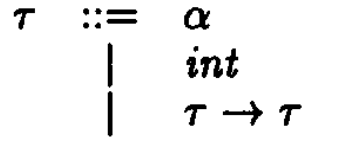
\includegraphics[scale=0.55]{paper_figure_1_tau.png} & 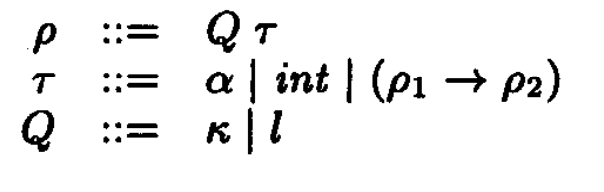
\includegraphics[scale=0.55]{paper_figure_3_no_label.png} \\
\hline

\includegraphics[scale=0.7]{paper_constraint_grammar.png} & 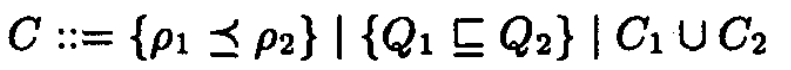
\includegraphics[scale=0.55]{paper_constraint_grammar_qualifs.png}\\
\hline
\end{tabular}
\renewcommand{\arraystretch}{1.0}

\bigskip
\pause

\textit{Q:} Why is there no $\rho_1 = \rho_2$ in the grammar for $C$?

\pause

\textit{A:} Because we can just use $\{\rho_1 \preceq \rho_2\} \cup \{\rho_2 \preceq \rho_1 \}$ instead.

\end{frame}

\begin{frame}{Constraint-Based Typing Rules With Qualifiers}

\infrule[Int]
{}
{A \ts n : int; \emptyset}

\infrule[Var]
{}
{A \ts x : A(x); \emptyset}

\infrule[Lam]
{\alpha \text{ fresh} ~~~~ \kappa \text{ fresh} ~~~~ A[x \rightarrow \kappa\alpha] \ts e : \rho_2 ; C}
{A \ts \lambda x . e : \kappa\alpha \rightarrow \tau_2 ; C}

\infrule[App]
{\alpha \text{ fresh} ~~~~ \kappa, \kappa' \text{ fresh} ~~~~ A \ts e_1 : \rho_1 ; C_1 ~~~~ A \ts e_2 : \rho_2 ; C_2}
{A \ts e_1 e_2 : \alpha ; C_1 \cup C_2 \cup \{ \rho_1 = \kappa(\rho_2 \rightarrow \kappa'\alpha) \}}

\infrule[If]
{\kappa \text{ fresh} ~~~~ A \ts e_1 : \rho_1; C_1 ~~~~ A \ts e_2 : \rho_2; C_2 ~~~ A \ts e_3 : \rho_3; C_3}
{A \ts \text{\textbf{if }} e_1 \text{\textbf{ then }} e_2 \text{\textbf{ else }} e_3 \text{\textbf{ fi}} : \rho_2;\\
 C_1 \cup C_2 \cup C_3 \cup \{\rho_1 = \kappa int\} \cup \{\rho_2 = \rho_3\}}

\infrule[Let]
{A \ts e_1 : \rho_1; C_1 ~~~~ A[x \rightarrow \rho_1] \ts e_2 : \rho_2; C_2}
{A \ts \text{\textbf{let }} x = e_1 \text{\textbf{ in }} e_2 \text{\textbf{ ni}} : \rho_2; C_1 \cup C_2}

\end{frame}

\begin{frame}{Question}

In an if-expression, what if the then-branch has type \texttt{const int} and the else-branch has type \texttt{int}: Can we still typecheck the expression?

\begin{itemize}
\item (If) rule from previous slide:

\infrule[]
{\kappa \text{ fresh} ~~~~ A \ts e_1 : \rho_1; C_1 ~~~~ A \ts e_2 : \rho_2; C_2 ~~~ A \ts e_3 : \rho_3; C_3}
{A \ts \text{\textbf{if }} e_1 \text{\textbf{ then }} e_2 \text{\textbf{ else }} e_3 \text{\textbf{ fi}} : \rho_2;\\
 C_1 \cup C_2 \cup C_3 \cup \{\rho_1 = \kappa int\} \cup \{ \rho_2 = \rho_3\}}

\pause

\item A better version:

\infrule[]
{\alpha, \kappa, \kappa' \text{ fresh} ~~~~ A \ts e_1 : \rho_1; C_1 ~~~~ A \ts e_2 : \rho_2; C_2 ~~~ A \ts e_3 : \rho_3; C_3}
{A \ts \text{\textbf{if }} e_1 \text{\textbf{ then }} e_2 \text{\textbf{ else }} e_3 \text{\textbf{ fi}} : \kappa'\alpha;\\
 C_1 \cup C_2 \cup C_3 \cup \{\rho_1 = \kappa int\} \cup \{ \rho_2 \preceq \kappa'\alpha \} \cup \{ \rho_3 \preceq \kappa'\alpha \}}
\end{itemize}

\end{frame}

\begin{frame}{Unification Algorithm}
\begin{itemize}

\item Reminder:
\begin{center}
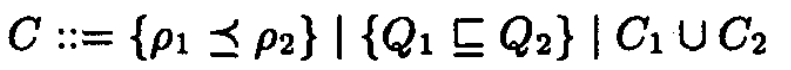
\includegraphics[scale=0.65]{paper_constraint_grammar_qualifs.png}
\end{center}

% \bigskip

\item \textbf{First phase:} Repeat
\begin{itemize}
\item $\{(Q_1\tau_1 \rightarrow Q_2\tau_2) \preceq (Q_3\tau_3 \rightarrow Q_4\tau_4)\} \cup C_{rest}$ \\
$\Rightarrow C_{rest} \cup \{Q_3\tau_3 \preceq Q_1\tau_1\} \cup \{ Q_2\tau_2 \preceq Q_4\tau_4\})$
\item $\{Q\tau \preceq Q'\tau\} \cup C_{rest} ~~\Rightarrow~~ C_{rest} \cup \{ Q \sqsubseteq Q'\}$
\item $\{Q\tau \preceq Q'\alpha\} \cup C_{rest} ~~\Rightarrow~~ [\alpha \rightarrow \tau]C_{rest} \cup \{Q \sqsubseteq Q'\}$
\item $\{Q\alpha \preceq Q'\tau\} \cup C_{rest} ~~\Rightarrow~~ [\alpha \rightarrow \tau]C_{rest} \cup \{Q \sqsubseteq Q'\}$
\end{itemize}
until only lattice constraints are left.

\item \textbf{Second phase:}\\
% \begin{itemize}
% \item 
All constraints now are of the form $\kappa \sqsubseteq L$, $L \sqsubseteq \kappa$, or $L_1 \sqsubseteq L_2$.\\
Solve in linear time as described in [HR97].
% \end{itemize}

\end{itemize}
\end{frame}

\begin{frame}{Step 3: Add Polymorphism}

Note: The goal is to be polymorphic in \emph{qualifiers}, not in \emph{types}.

\bigskip

\begin{center}
\renewcommand{\arraystretch}{1.5}
\begin{tabular}{|c | c|}
\hline
\textbf{Without polymorphism} & \textbf{With polymorphism} \\
\hline
$A$ contains $(x, \rho)$ tuples & $A$ contains $(x, \sigma)$ tuples\\
\hline

\includegraphics[scale=0.65]{paper_constraint_judgment_qualifs.png} & 
\includegraphics[scale=0.65]{paper_constraint_judgment_qualifs.png}\\
\hline  
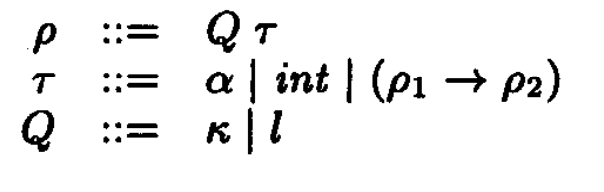
\includegraphics[scale=0.65]{paper_figure_3_no_label.png} & 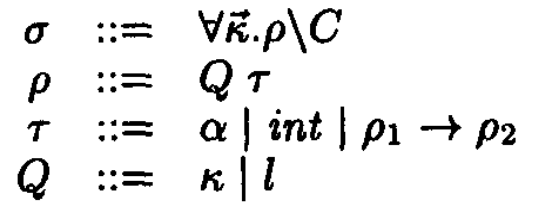
\includegraphics[scale=0.65]{paper_poly_types_grammar.png} \\
\hline
\end{tabular}
\renewcommand{\arraystretch}{1.0}
\end{center}

\bigskip

$\sigma$: Type scheme carrying constraints

\end{frame}

\begin{frame}[fragile]{Back to C: Example}

\begin{scriptsize}
\begin{lstlisting}[language=C,frame=none,belowskip=- \medskipamount]
const int * max_const(const int * p1, const int * p2) {
   if (*p1 < *p2) {
      return p2;
   } else {
      return p1;
   }
}

int * max_nonconst(int * p1, int * p2) { EXACTLY THE SAME BODY }

int main() {
   int v1 = 8;
   int v2 = 5;

   const int * p1_const = &v1;
   const int * p2_const = &v2;
   int bigger = *(max_const(p1_const, p2_const));
   printf("%d\n", bigger);
   
   int * p1_nonconst = &v1;
   int * p2_nonconst = &v2;
   int * p_bigger = max_nonconst(p1_nonconst, p2_nonconst);
   (*p_bigger)--;
}
\end{lstlisting}
\end{scriptsize}

\end{frame}

\begin{frame}[fragile]{Qualifier Polymorphism}

In C:

\begin{scriptsize}
\begin{lstlisting}[language=C,frame=none,belowskip=- \medskipamount]
const int * max_const(const int * p1, const int * p2)

int * max_nonconst(int * p1, int * p2)
\end{lstlisting}
\end{scriptsize}

\bigskip

Translated to the language of the paper:

\begin{scriptsize}
max\_const : $(\text{\textbf{const }} ref(\bot int)) \rightarrow (\text{\textbf{const }} ref(\bot int)) \rightarrow (\text{\textbf{const }} ref(\bot int))$

max\_nonconst : $(\bot ref(\bot int)) \rightarrow (\bot ref(\bot int)) \rightarrow (\bot ref(\bot int))$
\end{scriptsize}

\bigskip

Now with qualifier polymorphism:

\begin{scriptsize}
max: $\forall \kappa . (\kappa ref(\bot int)) \rightarrow (\kappa ref(\bot int)) \rightarrow (\kappa ref(\bot int)) \textbackslash \emptyset$
\end{scriptsize}

\end{frame}

\begin{frame}{Soundness}

Soundness = ``Nothing can go wrong during evaluation''

$\Longrightarrow$ Need to define evaluation rules

\end{frame}

\begin{frame}{Evaluation rules}
\begin{center}
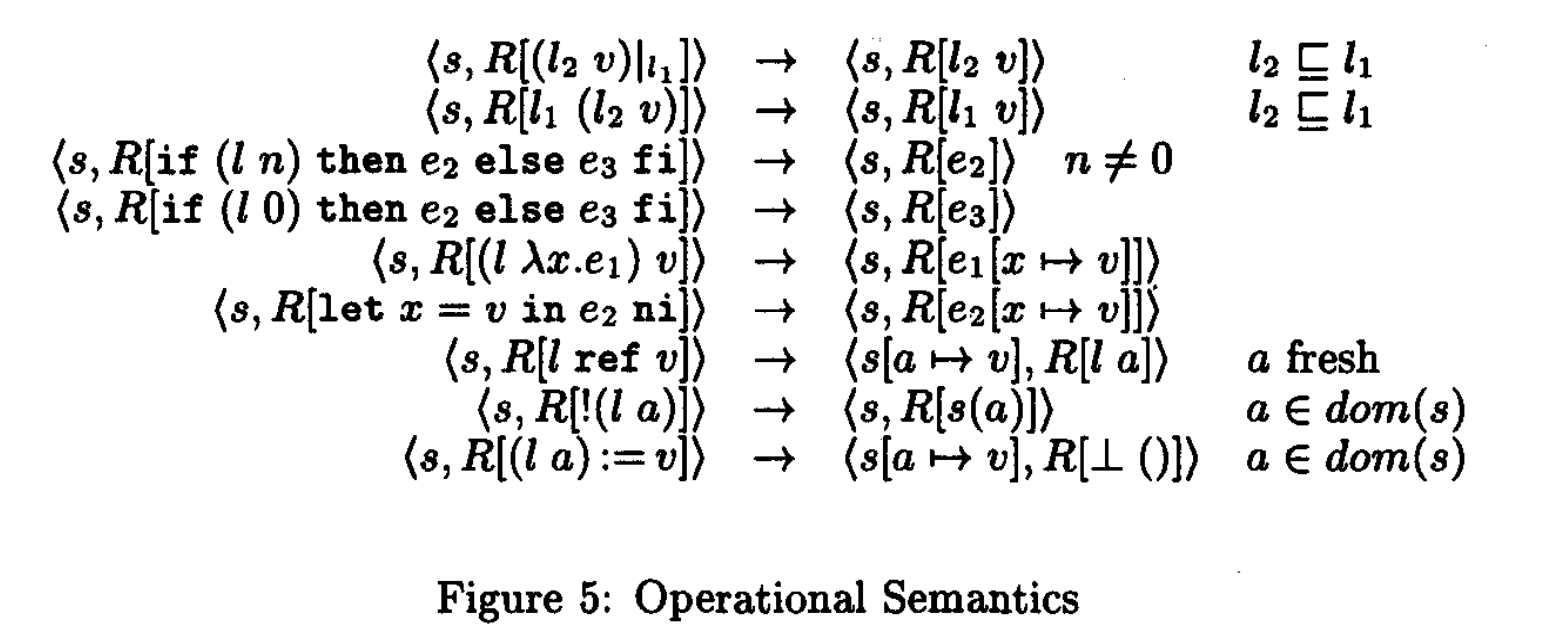
\includegraphics[scale=0.55]{paper_figure_5.png}
\end{center}
\end{frame}

\begin{frame}{Soundness}

TAPL: ``Soundness = Progress + Preservation''

Question: Where are these proofs in the paper?

\pause

Answer:
\begin{itemize}
\item Progress:\\
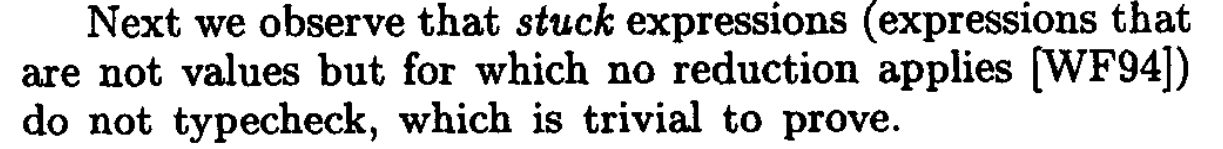
\includegraphics[scale=0.6]{paper_progress.png}
\item Preservation:\\
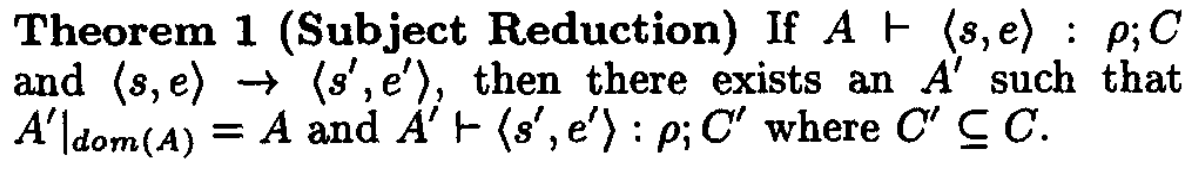
\includegraphics[scale=0.6]{paper_preservation.png}
\end{itemize}

\end{frame}

\begin{frame}{Helper lemmas for Subject Reduction}

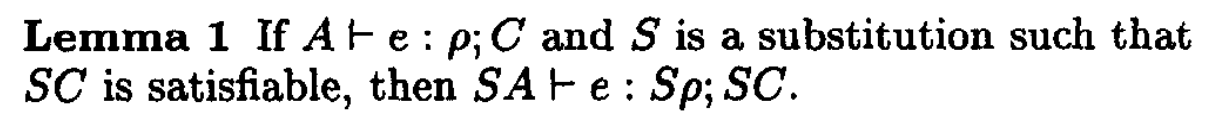
\includegraphics[scale=0.6]{paper_lemma_1.png}

\begin{itemize}
\item Question: What's the type of $S$?\\
\visible<2->{Answer: $TVar \rightarrow Typ$}

\item Question: Why is $S$ not applied to $e$?\\
\visible<3->{Answer: Because $e$ cannot contain type variables.}

\item Question: Don't we need another substitution lemma?\\
\visible<4->{Answer: Yes, we also need a substitution lemma on the term level, to prove that if we step from $(\lambda x . e_1) v$ to $e_1[x \rightarrow v]$, the type is preserved.}
\end{itemize}

\end{frame}

\begin{frame}{Soundness}

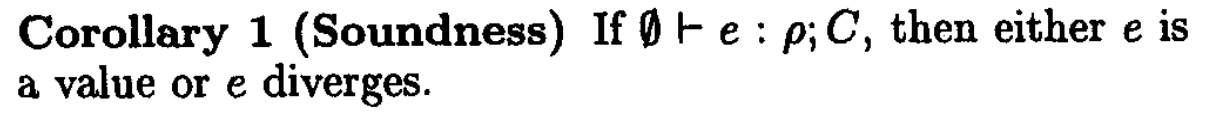
\includegraphics[scale=0.6]{paper_corollary_1.png}

Question: What does that mean? Isn't $(\lambda x.x)\,1$ a counterexample?

% no answer because we don't know it

\end{frame}

\begin{frame}{Benchmarks: Const Inference}

\begin{center}
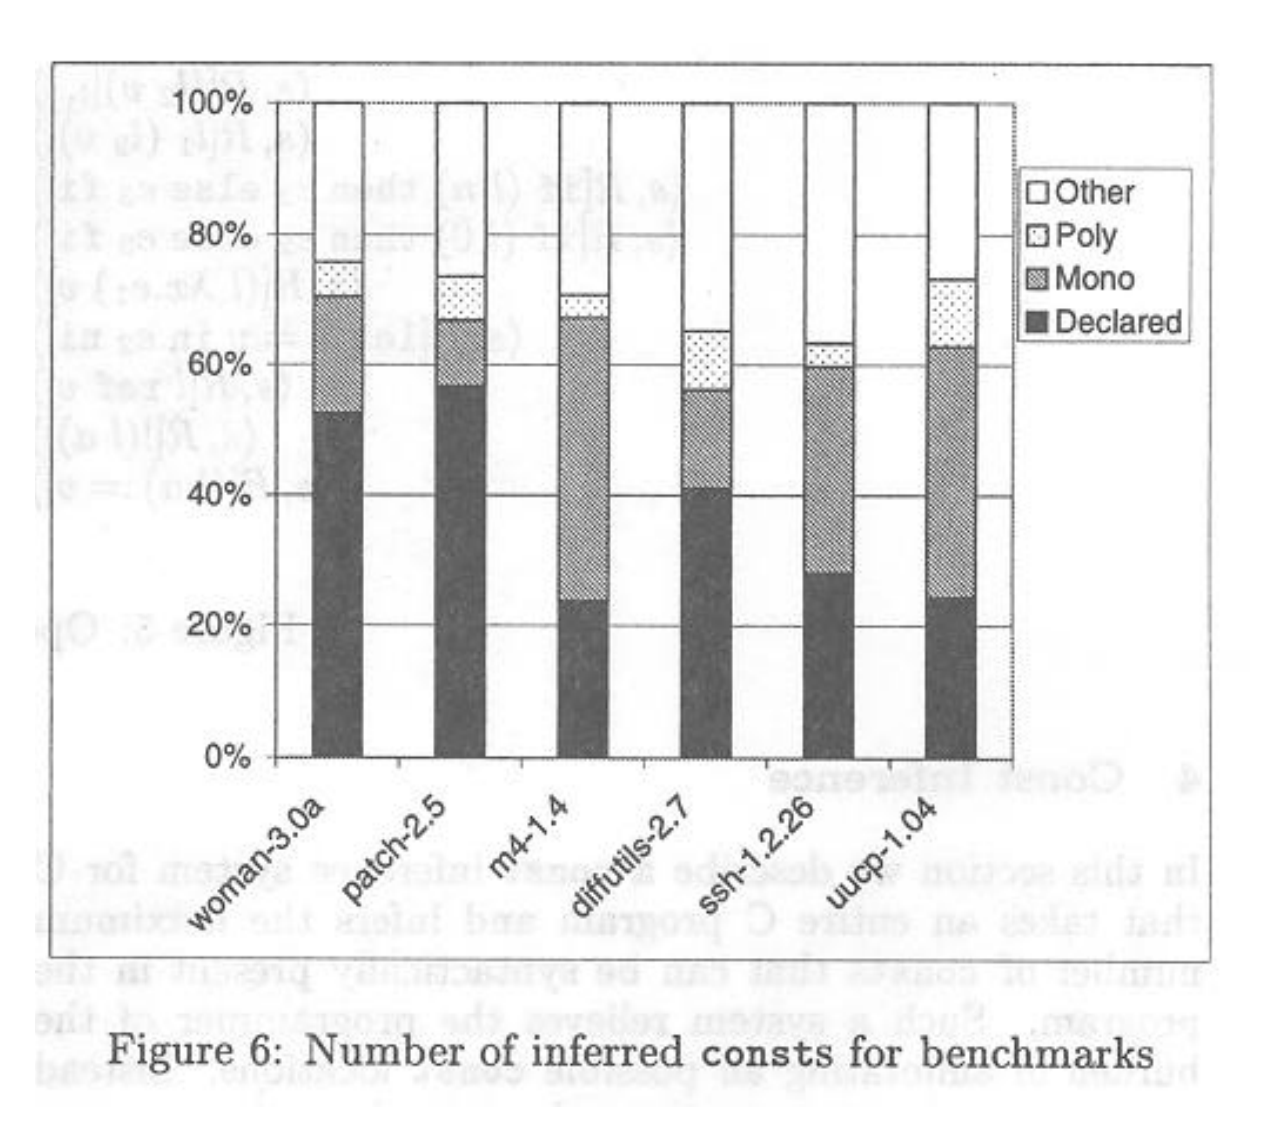
\includegraphics[scale=0.5]{paper_figure_6.png}
\end{center}

Question: What's the meaning of Other/Poly/Mono/Declared?

% give answer orally

\end{frame}

\begin{frame}{Discussion}

Question: What's the goal of qualifier inference?\pause
\begin{itemize}
\item Rewrite C source automatically?
\item More efficient program execution?
\item Make C qualifier-polymorphic?
\end{itemize}

\end{frame}

\begin{frame}
\begin{Huge}
\begin{center}
Thank you \smiley
\end{center}
\end{Huge}
\end{frame}


\end{document}
